% --------------------------------------------------------------------------- %
% Poster for HRI2017
% Vienna, Austria
% March 2017
% --------------------------------------------------------------------------- %
%
% Poster template reference
% http://www.brian-amberg.de/uni/poster/
%
% --------------------------------------------------------------------------- %


\documentclass[a0paper,portrait]{baposter}

\usepackage{calc}
\usepackage{graphicx}
\usepackage{amsmath}
\usepackage{amssymb}
\usepackage{relsize}
\usepackage{multirow}
\usepackage{rotating}
\usepackage{bm}
\usepackage{url}

\usepackage{graphicx}
\usepackage{multicol}

\newcommand{\captionfont}{\footnotesize}

\graphicspath{{images/}{../images/}}
\usetikzlibrary{calc}

\newcommand{\SET}[1]  {\ensuremath{\mathcal{#1}}}
\newcommand{\MAT}[1]  {\ensuremath{\boldsymbol{#1}}}
\newcommand{\VEC}[1]  {\ensuremath{\boldsymbol{#1}}}
\newcommand{\Video}{\SET{V}}
\newcommand{\video}{\VEC{f}}
\newcommand{\track}{x}
\newcommand{\Track}{\SET T}
\newcommand{\LMs}{\SET L}
\newcommand{\lm}{l}
\newcommand{\PosE}{\SET P}
\newcommand{\posE}{\VEC p}
\newcommand{\negE}{\VEC n}
\newcommand{\NegE}{\SET N}
\newcommand{\Occluded}{\SET O}
\newcommand{\occluded}{o}

\usepackage{enumitem}% http://ctan.org/pkg/enumitem

\usepackage[utf8]{inputenc}
%Ionuţ-Alexandru Zaiţi, Ştefan-Gheorghe Pentiuc, Radu-Daniel Vatavu
%http://www.latex-community.org/forum/viewtopic.php?f=31&t=9084


%%%%%%%%%%%%%%%%%%%%%%%%%%%%%%%%%%%%%%%%%%%%%%%%%%%%%%%%%%%%%%%%%%%%%%%%%%%%%%%%
%%%% Some math symbols used in the text
%%%%%%%%%%%%%%%%%%%%%%%%%%%%%%%%%%%%%%%%%%%%%%%%%%%%%%%%%%%%%%%%%%%%%%%%%%%%%%%%

%%%%%%%%%%%%%%%%%%%%%%%%%%%%%%%%%%%%%%%%%%%%%%%%%%%%%%%%%%%%%%%%%%%%%%%%%%%%%%%%
% Multicol Settings
%%%%%%%%%%%%%%%%%%%%%%%%%%%%%%%%%%%%%%%%%%%%%%%%%%%%%%%%%%%%%%%%%%%%%%%%%%%%%%%%
\setlength{\columnsep}{1.5em}
\setlength{\columnseprule}{0mm}

%%%%%%%%%%%%%%%%%%%%%%%%%%%%%%%%%%%%%%%%%%%%%%%%%%%%%%%%%%%%%%%%%%%%%%%%%%%%%%%%
% Save space in lists. Use this after the opening of the list
%%%%%%%%%%%%%%%%%%%%%%%%%%%%%%%%%%%%%%%%%%%%%%%%%%%%%%%%%%%%%%%%%%%%%%%%%%%%%%%%
\newcommand{\compresslist}{%
\setlength{\itemsep}{1pt}%
\setlength{\parskip}{0pt}%
\setlength{\parsep}{0pt}%
}

%%%%%%%%%%%%%%%%%%%%%%%%%%%%%%%%%%%%%%%%%%%%%%%%%%%%%%%%%%%%%%%%%%%%%%%%%%%%%%
%%% Begin of Document
%%%%%%%%%%%%%%%%%%%%%%%%%%%%%%%%%%%%%%%%%%%%%%%%%%%%%%%%%%%%%%%%%%%%%%%%%%%%%%

\begin{document}

%%%%%%%%%%%%%%%%%%%%%%%%%%%%%%%%%%%%%%%%%%%%%%%%%%%%%%%%%%%%%%%%%%%%%%%%%%%%%%
%%% Here starts the poster
%%%---------------------------------------------------------------------------
%%% Format it to your taste with the options
%%%%%%%%%%%%%%%%%%%%%%%%%%%%%%%%%%%%%%%%%%%%%%%%%%%%%%%%%%%%%%%%%%%%%%%%%%%%%%
% Define some colors

% \definecolor{lightblue}{cmyk}{0.83,0.24,0,0.12}
\definecolor{lightblue}{rgb}{0.145,0.6666,1}

\definecolor{bgc_1}{RGB}{93, 194,232}
\definecolor{bgc_2}{RGB}{144, 190, 242}


\definecolor{hc_1}{RGB}{29,105,218}
\definecolor{hc_2}{RGB}{240,141,96}


\hyphenation{perform repetitions comfortable provides recognition triaxial}

%%
\begin{poster}%
  % Poster Options
  {
  % Show grid to help with alignment
  grid=false,
  % Column spacing
  colspacing=1em,
  % Color style
  bgColorOne=white,
  bgColorTwo=white,
  borderColor=lightblue,
  headerColorOne=black,
  headerColorTwo=lightblue,
  headerFontColor=white,
  boxColorOne=white,
  boxColorTwo=lightblue,
  % Format of textbox
  textborder=roundedleft,
  % Format of text header
  eyecatcher=true,
  headerborder=closed,
  headerheight=0.125\textheight,
%  textfont=\sc, An example of changing the text font
  headershape=roundedright,
  headershade=shadelr,
  headerfont=\Large\bf\textsc, %Sans Serif
  textfont={\setlength{\parindent}{1.5em}},
  boxshade=plain,
%  background=shade-tb,
  background=plain,
  linewidth=2pt
  }
%%% Eye Cacther %%%%%%%%%%%%%%%%%%%%%%%%%%%%%%%%%%%%%%%%%%%%%%%%%%%%%%%%%%%%%%%
{
	Eye Catcher, empty if option eyecatcher=false - unused
%    \includegraphics[height=3em]{conacyt_logo_v1.png}
}
%%% Title %%%%%%%%%%%%%%%%%%%%%%%%%%%%%%%%%%%%%%%%%%%%%%%%%%%%%%%%%%%%%%%%%%%%%
{\bf
  {Towards the Quantification of Human-Robot Imitation \\ Using Wearable Inertial Sensors}
}
%%% Authors %%%%%%%%%%%%%%%%%%%%%%%%%%%%%%%%%%%%%%%%%%%%%%%%%%%%%%%%%%%%%%%%%%%
{
	%\vspace{-0.3em} 
	{\smaller {Miguel P. Xochicale\textsuperscript{1}, 
	Chris Baber\textsuperscript{1} and 
	Mourad Oussalah\textsuperscript{2}}; [map479@bham.ac.uk]  } \\ 
	%\vspace{-0.5em}
	{\smaller
	\textsuperscript{1} School of Electronic, Electrical and Systems Engineering, University of Birmingham, UK \\
	\textsuperscript{2} Center for Ubiquitous Computing, University of Oulu, Finland }
}
% % Logos
%   {% The makebox allows the title to flow into the logo, this is a hack because of the L shaped logo.
%   	\fbox{
%     \begin{minipage}{11em}
%     
%       \begin{center}
%       \includegraphics[height=2.7em]{conacyt_logo_v1}\\
%       \includegraphics[height=2.95em]{uob_logo} \\
%       \includegraphics[height=1.8em]{University_of_Oulu_logo}  
%       \end{center}
%       
%     \end{minipage}
%       }
%   } 


%%%%%%%%%%%%%%%%%%%%%%%%%%%%%%%%%%%%%%%%%%%%%%%%%%%%%%%%%%%%%%%%%%%%%%%%%%%%%%
%%% Now define the boxes that make up the poster
%%%---------------------------------------------------------------------------
%%% Each box has a name and can be placed absolutely or relatively.
%%% The only inconvenience is that you can only specify a relative position 
%%% towards an already declared box. So if you have a box attached to the 
%%% bottom, one to the top and a third one which should be in between, you 
%%% have to specify the top and bottom boxes before you specify the middle 
%%% box.
%%%%%%%%%%%%%%%%%%%%%%%%%%%%%%%%%%%%%%%%%%%%%%%%%%%%%%%%%%%%%%%%%%%%%%%%%%%%%%
    %
    % A coloured circle useful as a bullet with an adjustably strong filling
    \newcommand{\colouredcircle}{%
      \tikz{\useasboundingbox (-0.2em,-0.32em) rectangle(0.2em,0.32em); 
      \draw[draw=black,fill=lightblue,line width=0.03em] (0,0) circle(0.18em);}}

      
      
      
\headerbox{Objectives}{name=rq,span=2,column=0,row=0}{
% \& Research Question
For this study, we are proposing a framework based on Nonlinear Dynamics
in order to explore a metric that can help us to determine
how close humans mimic the movement of a robot with the use of wearable 
inertial sensors.

% How to analyse  data collected from wearable inertial sensors attached both 
% to a person and to a humanoid robot in order to quantify how closely a participant 
% imitates a robot.



}


\headerbox{Background}{name=intro,span=2,column=0,below=rq}{

NAO, a humanoid robot, has successfully been used both as a fitness coach for the elderly 
and as an instructor of rehabilitation for children.

For instance, G{\"{o}}rer et al. \cite{gorer2016} used NAO as an exercise tutor 
and an Asus Xtion RGB-D camera to get the 
% which were employed to extract the joint angles of a human demonstrator and some participants. 
absolute differences of the joint angles between the human demonstrator and the participants
which were used to create a corrective feedback for the movement of the elderly.
% with respect to (i) speed adjustment, (ii) amplitude adjustment, (iii) mirroring detection, and (iv) motion.
However, when participants are seated, the RGB-D camera cannot provide correct skeletal information of the participant.

Similarly, Guneysu et al. \cite{guneysu2015} used NAO and wearable inertial sensors to monitor 
the motions of arm rehabilitation of children.
However, it was revealed that the four physiotherapists all moved in 
slightly different ways while performing the same arm motions; which is reflected in the differences 
of frequency and amplitude of the movements as well as in the initial positions of their hands.

% The challenge for Guneysu et al. was to keep the children motivated in order to imitate 
% movements for arm rehabilitation therapy. 



}


\headerbox{Methods}{name=methods,span=2,column=0,below=intro}{

Twelve right-handed healthy participants (two females and ten males) with a mean age 
of 19.5$\pm$0.79 (abbreviated as p01 to p12) were 
% invited to participate in this study. 
% Participants were 
asked to imitate, in a front to front activity, simple horizontal and vertical arm movements performed by NAO.


Data were collected at a sampling rate of 50Hz with two NeMEMSi inertial sensors
which provide tri-axial data of accelerometer, gyroscope and magnetometer sensors and
quaternions \cite{comotti2014}.
}




\headerbox{State Space Reconstruction (SSR)}{name=ssr,span=2,column=0,below=methods}{

\begin{tabular}{ccc}


\begin{minipage}{0.37\textwidth}

The state space reconstruction  is based on the methods of time-delay embedding and PCA \cite{gibson1992}.
The method of time-delay embedding is an array of 
delayed copies of the available time series $x(n)$ and is defined as  
$ \overline{x}(n) = \{  x(n), x(n-\tau), x(n-2\tau), \dots,x(n-(m-1)\tau)\}$;
where $m$ is the embedding dimension and $\tau$ is the delay embedding.

Our motivation to use the method of time-delay embedding 
is due to the nonlinear structure of the time-series which is 
presented as different periods and amplitudes of the time-series 
between repetitions of movements and across movements of participants

\end{minipage}


\begin{minipage}{0.5\textwidth}

\begin{center}
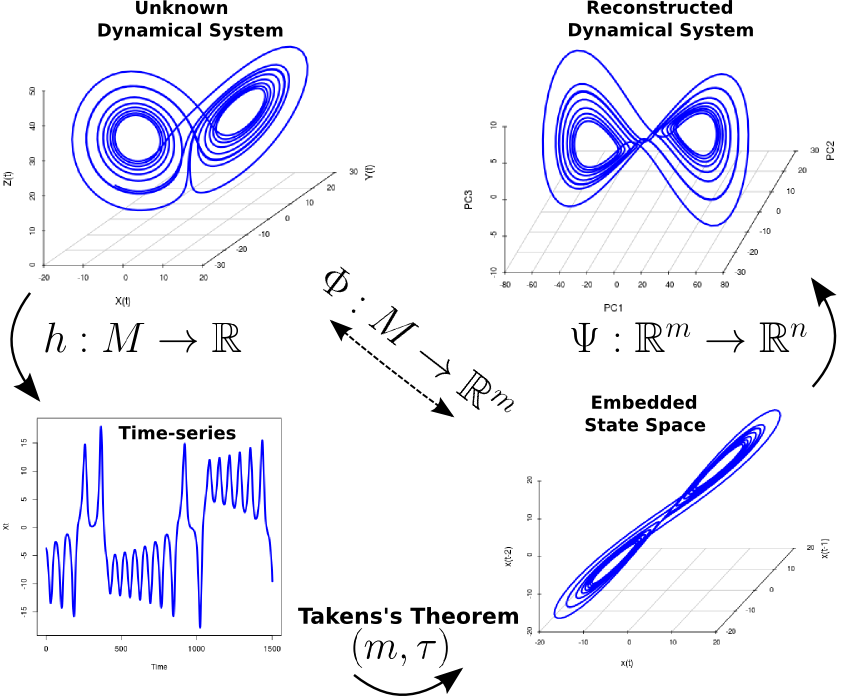
\includegraphics[width=1.1\textwidth]{takens_theorem_v5.png}  
\end{center}

\end{minipage}



\end{tabular}



}

\headerbox{Conclusion and Outlook}{name=conclusion,span=2,column=0,below=ssr}{



It can be noted that participants show different ranges of imitation which 
can be linked to a scoring system of human-robot imitation.
However, the quality of such metric is debatable and needs further investigation.
Therefore, there are four areas that we intent to investigate:
\begin{itemize}[noitemsep,topsep=0pt]
 \item Data collection from a wider range of individuals 
 (differing gender, age and state of health) and from additional inertial sensors attached to the body;
 \item Exploration of complex movements which can be performed by both persons and NAO;
\item Undertake a wider review of nonlinear dynamics techniques that can be used for 
the assessment of human-robot imitation; and, 
 \item Exploration of deep neural networks for automatic classification of the levels of imitation.
\end{itemize}



%
%   \item How can the time-delay embedding and PCA methods quantify the variability of human activities?
% \end{itemize}
%\vspace{1.5mm}

}

  
%%%%%%%%%%%%%%%%%%%%%%%%%%%%%%%%%%%%%%%%%%%%%%%%%%%%%%%%%%%%%%%%%%%%%%%%%%%%%%
\headerbox{References}{name=references,span=2,column=0,below=conclusion,above=bottom}{
%%%%%%%%%%%%%%%%%%%%%%%%%%%%%%%%%%%%%%%%%%%%%%%%%%%%%%%%%%%%%%%%%%%%%%%%%%%%%%
     \smaller
    \vspace{-0.4em} % Save some space at the beginning
    \bibliographystyle{ieee}
    \renewcommand{\section}[2]{\vskip 0.05em}

\begin{thebibliography}{1}
\itemsep=-0.01em
\setlength{\baselineskip}{0.4em}

\bibitem{gorer2016}
B. G{\"{o}}rer, A. A. Salah and H.L Akin.
\newblock An autonomous robotic exercise tutor for elderly people.
\newblock In {\em Autonomous Robots}, (July), 2016.


\bibitem{guneysu2015}
A. Guneysu and B. Arnrich.
\newblock Children's Rehabilitation with Humanoid Robots and Wearable Inertial Measurement Units.
\newblock In {\em 9th IEEE International Conference on Pervasive Computing Technologies for Healthcare}, pages 7-10, 2015.



\bibitem{comotti2014}
D. Comotti, M. Galizzi and A. Vital.
\newblock NeMEMSi: One step forward in wireless attitude and heading reference systems.
\newblock In {\em 1st IEEE International Symposium on Inertial Sensors and Systems}, 1-4,2014

\bibitem{gibson1992}
J. F. Gibson, J. D. Farmer, M. Casdagli and S. Eubank.
\newblock An analytic approach to practical state space reconstruction
\newblock In {\em Physica D: Nonlinear Phenomena}, 1-30, 1992.


  

\end{thebibliography}
}


%,above=bottom
\headerbox{Results}{name=results,span=1,column=2,row=0,aligned=rq}{

The robot's performance was highly consistent as indicated by the blue lines in time-series 
and by the tight circular shape in the state space.
Compared with the consistency of the robot, p01 was able to imitate the robot's movement 
well by maintained a good level of consistency as shown both by the time-series and by the circular shape in the SSR.
The other participant here, p05, had some problems in following the robot.
This is shown by the red line in time-series and the disjointed circular shape 
of the  state space.

One  can see that participants p02, p05, p07, and p12 seemed
to have more difficulty than others in maintaining a consistent response
to the robot's movement.

% The values for percentage cumulative energy (PCE) from five participants 
% are presented using boxplots for both low-cost and commercial triaxial accelerometer (ACC).
% It is visually evident that both sensors present similar results for each movement.
% It is highlighted that the circular movement shows the least variation 
% per component compare to other movements. 
% 
% We assume that the evident variability of the movements 
% is due to the flexibility in the experiment where participants
% were only asked to perform the movements at a comfortable speed.


% \vspace{-4mm}
\begin{center}
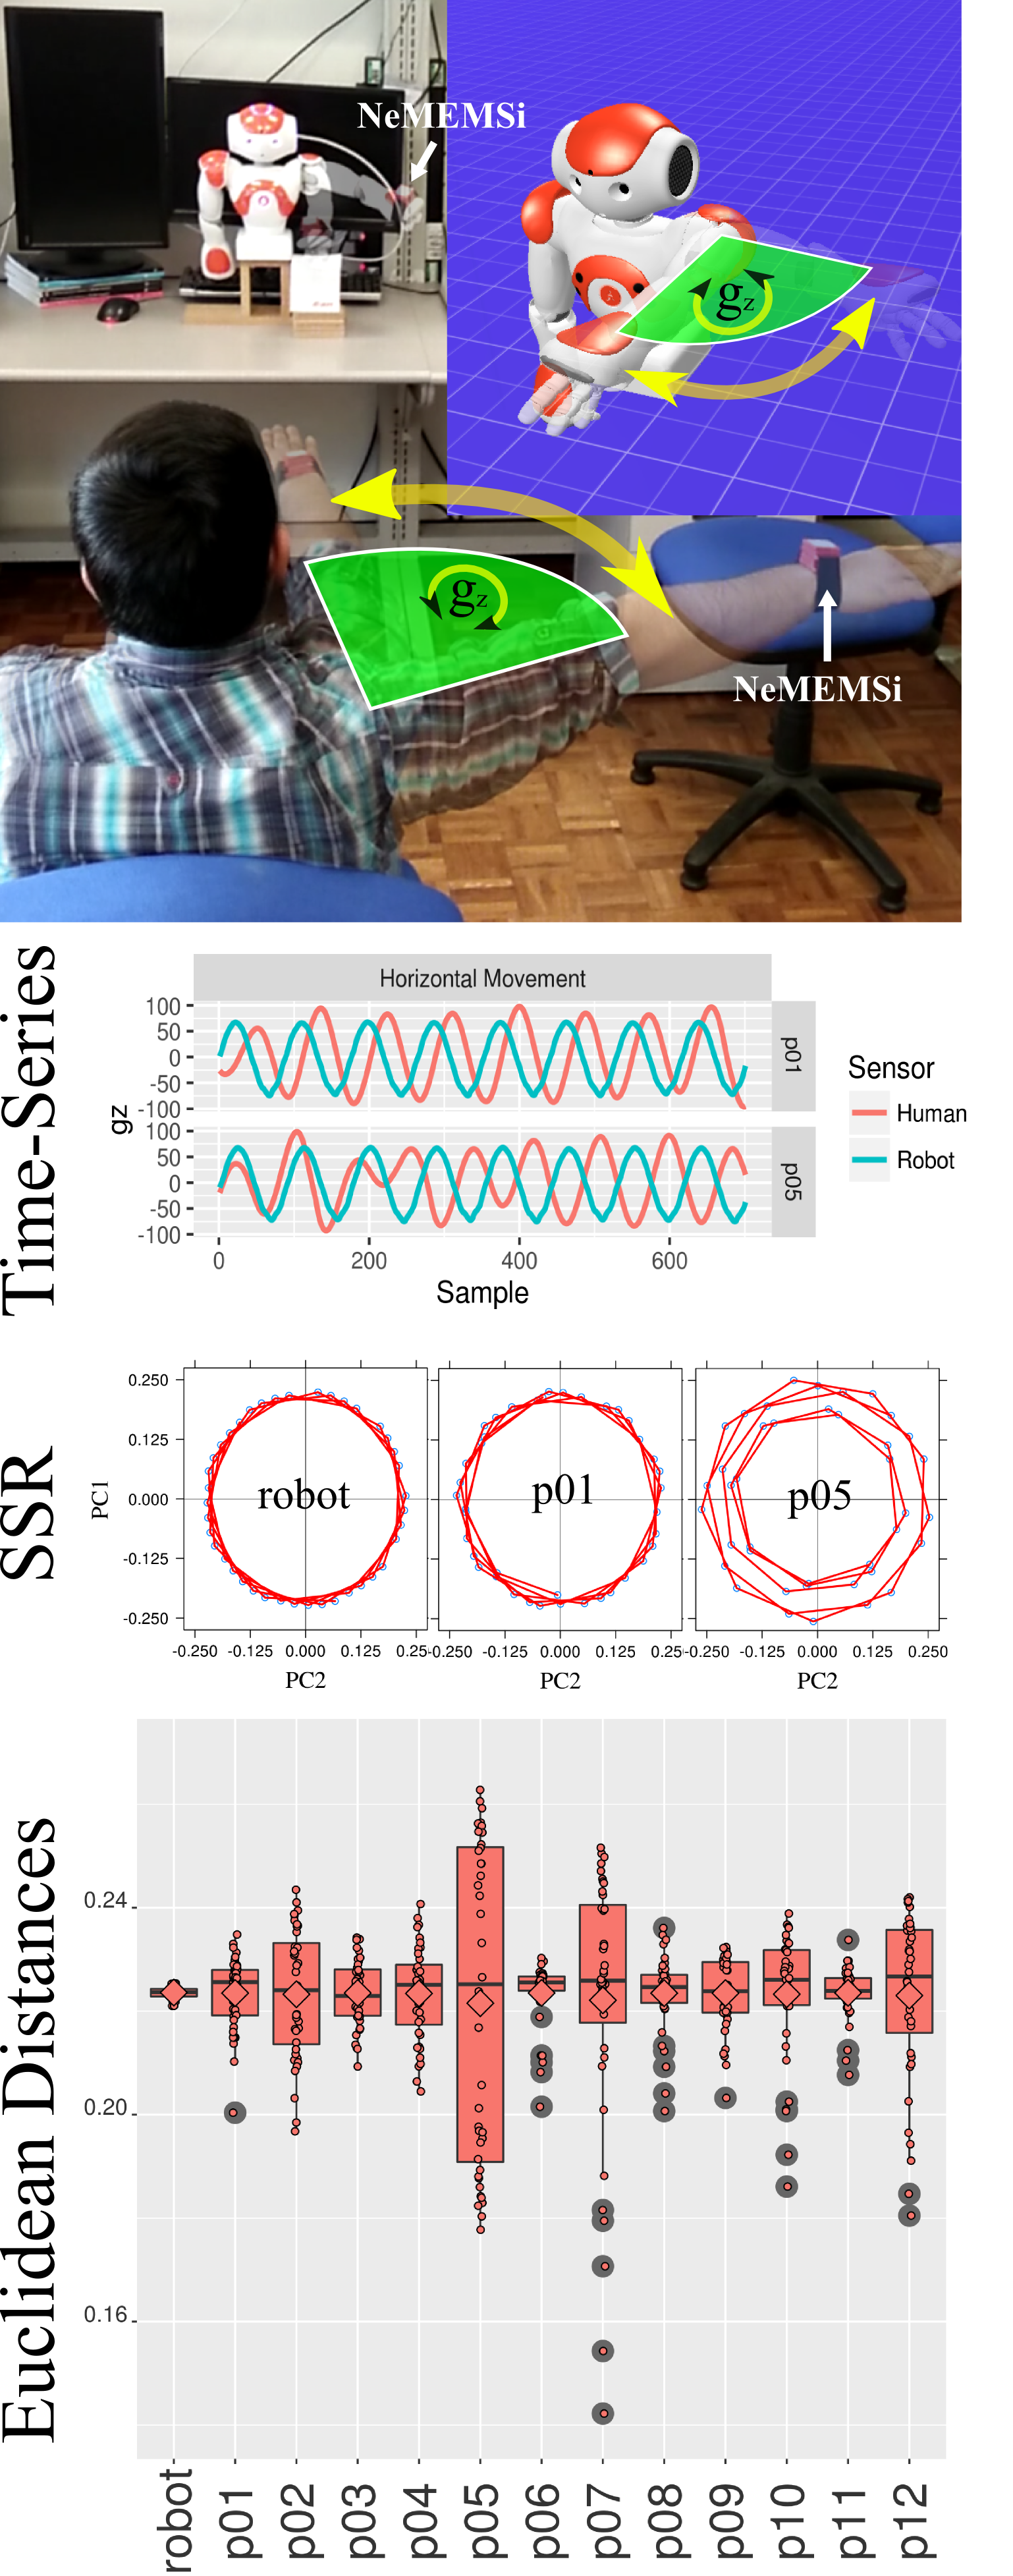
\includegraphics[width=0.97\linewidth]{mainfig03} 
\end{center}


}


\headerbox{Acknowledgements}{name=acknowledgements,span=1,column=2,row=0,above=bottom}{

Miguel P. Xochicale gratefully acknowledges the studentship 
from the National Council for Science and Technology (CONACyT) Mexico for pursuing his doctoral
studies at The University of Birmingham, UK.
}


  

\end{poster}

\end{document}
